\documentclass[11pt]{article}

%\usepackage{deauthor}

%\usepackage{times}

%\usepackage[pdftex]{graphicx}
%\DeclareGraphicsExtensions{.pdf,.jpeg,.jpg,.png}
%\graphicspath{{soumagne/}}

%\usepackage[affil-it]{authblk}
%\setlength{\affilsep}{0em}

%\usepackage[labelfont=bf,labelsep=space,list=true]{subcaption}

%\usepackage{url}

\begin{document}
\title{Advancing RPC for Data Services at Exascale}
\author[1]{Jerome Soumagne}
\author[2]{Philip Carns}
\author[2]{Robert B. Ross}
\affil[1]{The HDF Group}
\affil[2]{Argonne National Laboratory}

\maketitle

\begin{abstract}
Remote Procedure Call (RPC) has long been an inherent component of parallel
file systems and I/O forwarding middleware in high-performance computing
(HPC).  RPCs are used in this environment to issue
I/O operations and transfer data from compute nodes to gateway and server storage
nodes. With HPC systems becoming more heterogeneous, data volumes
reaching new thresholds, and I/O standing as the main bottleneck, there is a growing
need in the HPC community to build distributed services and adopt new workflows
that are, nonetheless, no longer dictated by monolithic parallel file systems. These include
specialized storage, data analysis, and telemetry
services that can be adapted to fit application needs. Parallel file system
RPC facilities have never been exposed to service or middleware developers,
however, leaving them with two choices: MPI or the low-level fabric network
protocol.
In this article, we show how an independent RPC framework can be used as a building block for
developing user-level data services at exascale. We identify the design
choices that must be considered in terms of both performance and resilience
for HPC
data services, and we discuss the directions taken to palliate current HPC system constraints.
\end{abstract}

\section{Introduction}
\label{sec:intro}

High-performance computing (HPC) facilities have traditionally
been designed around \textit{monolithic} file systems, which are tailored to
scientific HPC workflows comprised of computation, storage, and
data analysis. Scientific application users, whose needs depend
on the application's domain, have been constrained to conform to system precepts
and this standard workflow. While this has been
a viable (but increasingly limiting) option for pre-exascale systems,
increasing data volumes and increasing system complexity with
emerging hardware are now forcing application users to adopt new
\textit{specialized} workflows.  These specialized workflows not only achieve sustainable
performance and perform data analysis in a timely manner at an increasing
scale, but also better respond to application needs and provide data
insights, for example through monitoring and telemetry service.

Creating specialized workflows requires the introduction of
a collection of \textit{data services} to the HPC ecosystem that must interact
with both the
system components (hardware and software) and the application.
While some of those services may be provided by the system, the vast majority
of data services are user-level services that are developed to augment the
original HPC system software stack and better serve the application's
performance or functionality needs. Data services (system-provided
or user-provided) must respond, in most cases, to the same user
prerequisites by ensuring performance, resilience, and ease of deployment.
These prerequisites introduce engineering challenges that
must be overcome when creating a new HPC data service---by no means an
easy task. One such challenge is communication: data exchange
between services is a critical aspect of
specialized workflows that are composed of multiple services interacting with
each other. Developing the messaging part of a data service component on an HPC
machine can, for a new service developer, involve either using the
low-level network fabric
API, which requires a significant amount of work and expertise, or using the vendor installed
MPI library~\cite{mpich} that takes advantage of the underlying network fabric. 
MPI itself, however, is not very suitable for developing such dynamical services that
may come and go
%, nor is it suitable for efficiently accessing memory of a remote process
%without prior collective synchronization
~\cite{Zounmevo2013}.
%
MPI implementations have consistently prioritized use
by applications and not by service libraries.

Data services are already a well-established technology in the cloud, where
remote procedure call (RPC) is the main technique used for sending messages
to remote components. Google gRPC~\cite{protobuf} or Facebook Thrift~\cite{Slee2007}
are good examples of such
frameworks. However, they are not well-suited to run on HPC systems because they (1)
rely on the TCP/IP stack and do not take advantage of the low latency/high
bandwidth HPC fabrics and (2) are not designed for exchanging very large amounts
of data, a task that is left to the user.
In contrast, RPC has been used as the communication pillar of
distributed file systems (e.g., Lustre Networking (LNET)~\cite{Wang2009},
Panasas~\cite{Welch2008}) and I/O forwarding layers
(e.g., IOFSL~\cite{Ali2009}) that are specifically designed to send I/O requests on top of the
underlying network fabric. The Network File System (NFS)~\cite{Sandberg1988}
is also a good example of the use of RPC with large data transfers and
therefore close to the use of RPC in an HPC system.
The internal RPC facilities of these file systems (with the exception of NFS) have,
nonetheless, never
been directly exposed to users; instead, they have been deeply buried in the
monolithic file system software stacks that often extend into kernel space.
Other parallel file systems have implemented their own network abstraction layer
to support multiple network fabrics
and provide messaging capabilities that can support data services. However, they are not
general-purpose RPC frameworks, and in most cases cannot be easily extracted
from the file systems that they were designed for.

Based on both of those technologies and past experience with I/O forwarding,
we introduced in~\cite{Soumagne2013} an RPC framework, called Mercury, that takes
advantage of low-level HPC network fabrics and facilitates the development
of user-level data services. Mercury is part of a more comprehensive suite of components named
Mochi~\cite{Ross2020} that provides
a collection of service components for the creation of specialized data services.
We present in this paper how some of the design
choices made for Mercury are essential for building an heterogeneous service
workflow in an exascale HPC environment. In Section~\ref{sec:related}, we
present some of the work that
is similar to Mercury and approaches that we take to develop user-level data
services. In Section~\ref{sec:overview}, we give a brief overview of Mercury's
architecture before focusing in Section~\ref{sec:design} on the specific design
points that make an RPC framework usable for HPC data services, supporting our
claims by evaluation results. In Section~\ref{sec:apps}, we present some of the data services that are
successfully being deployed using Mochi and Mercury.
In Section~\ref{sec:concl}, we summarize our conclusions.

\section{Related Work}
\label{sec:related}

A few other frameworks and suites of HPC data service components have been proposed
using an approach similar to the one we used in Mercury. We present here
three of the most notable frameworks.

\textit{DataSpaces}~\cite{Docan2012} implements a
scalable, semantically specialized shared-space abstraction that is
dynamically accessible by all components and services in an application
workflow, supporting both application/system-aware data placement and data movement.
It relies on the \textit{Decoupled and Asynchronous Remote Transfers} (DART)~\cite{Docan2010}
layer, which is not defined as an explicit RPC framework, although it allows transfer of
large amounts of data using a client/server model from applications running on
the compute nodes of an HPC system to local storage or remote locations, in
order to enable remote application monitoring, data analysis, code coupling,
and data archiving.
The key requirements that DART seeks to satisfy are minimizing data transfer
overheads on the application; achieving high throughput, low latency data
transfers; and preventing data losses. To this end, DART is
designed so that dedicated nodes (i.e., separate from the application compute
nodes) asynchronously extract data from the memory of the compute nodes using
remote direct memory access (RDMA).

The \textit{Scalable Observation System} (SOSflow)~\cite{Wood2016} provides a broad
set of online and in situ capabilities, including code steering via remote method
invocation, data analysis, and visualization. SOSflow can couple together
multiple sources of data, such as application components and operating
environment measures, with multiple software libraries and performance
tools. SOSflow's communication mechanism relies both on TCP sockets for
on-node communication and on MPI for off-node communication. Its main communication
pattern is a publish-and-subscribe mechanism and relies on a daemon that is
launched as a background  process  in  user space at the start of a
job script, before the scientific workflow begins.

\textit{Faodel}~\cite{Ulmer2018} provides a set of services for data
management and exchange in HPC workflows. Three major components of
Faodel are Kelpie, Opbox, and Lunasa. Kelpie provides a key-blob
abstraction. OpBox is a library for implementing asynchronous communication
between multiple entities in a distributed application, and provides the user
with primitives for expressing a protocol as a state machine that the
communication layer can process in an asynchronous manner. It also provides
a naming service to locate components of an application. Lunasa provides
user-level network memory management services and effectively
acts as a memory registration cache for doing RDMA. Faodel relies on
an evolution of the NNTI layer from the \textit{NEtwork Scalable
Service Interface} (Nessie)~\cite{Lofstead2011} RPC library.
It provides an asynchronous RPC solution, designed to overlap computation and
I/O. Nessie also provides a mechanism to handle bulk data transfers, which can use
RDMA to transfer data efficiently from one memory to the other, and supports
several network transports. Nessie uses the RPC interface to push
control messages to the servers and exposes a separate one-sided API that is
used to push or pull data between client and server.

\section{Overview and Considerations}
\label{sec:overview}

Mercury is designed around three key paradigms: provide reliable RPC
functionality, support large data arguments, and take advantage of the HPC network
fabrics. In terms of functionality, much more is needed when
developing distributed HPC data services; but as opposed to RPC frameworks that are
part of monolithic software stacks, Mercury remains as thin as possible
in order to allow for reusability between various service components that must
support different needs.

\begin{figure}[h]
\centering
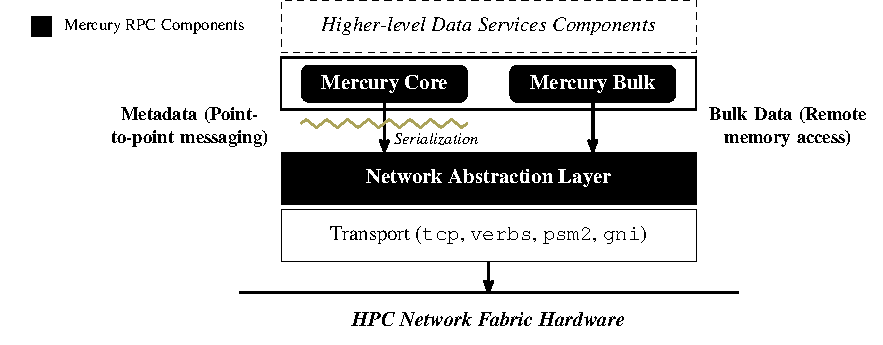
\includegraphics{figs/overview}
%\vspace{-5pt}
\caption{Overview of Mercury RPC components in the software stack.}
\label{fig:overview}
%\vspace{-10pt}
\end{figure}

As shown in Figure~\ref{fig:overview}, Mercury is composed of
two service-level components:
a core RPC component, which is designed to serialize
function arguments and send them to a remote target for execution using
point-to-point messaging, and a bulk
component, which is designed to handle large arguments (i.e., arguments that are
generally larger than 4KB depending on the underlying protocol being used).
This latter component enables the creation of
memory descriptors that can be sent along with the other arguments to the RPC
target to initiate raw memory transfers (without serialization) using remote memory access (RMA).
In Section~\ref{sec:rdma}, we detail this scenario and its benefits.
%
In order to support a large variety of HPC network fabrics,
both of these components interface with a network abstraction
layer that provides a minimum set of network primitives for both
point-to-point messaging and one-sided RMA communication operations.
Moreover, in order to reduce the burden of connection handshakes
when the underlying network does not necessarily request it (also
essential for scalability) and to support services that may come and go,
remote peers are addressed through unconnected endpoints.
Furthermore, in order to maximize throughput, all communication is made
nonblocking through a callback-based approach that we detail in
Section~\ref{sec:cb}.

While these points describe the overall architecture of an RPC
framework for HPC, additional key items can rapidly become prerequisites for
creating an RPC framework that is designed to support data services. These
include maximizing throughput, providing scaling, 
enabling flexibility, and ensuring resilience. In the
following section we describe how one can enhance RPC to (1) leverage RDMA-capable networks;
(2) support node-local service scaling and leverage multi-core processors;
(3) enable flexible, node-local deployment scenarios and service 
composition; (4) bridge nodes between multiple HPC networks; (5) enable fault tolerance.

\section{Enabling RPC for HPC Data Services}
\label{sec:design}

We do not compile an exhaustive list of features in this section.
%
Instead, we focus on those features that are necessary to enable strong service scaling,
performance, flexibility, and resilience for data services on emerging
large-scale computing platforms.

\subsection{HPC Network Support}
\label{sec:rdma}

As opposed to cloud-based RPC solutions that rely on TCP networking,
HPC network fabrics provide dedicated solutions that offer both
low latency and high bandwidth. To take advantage of these solutions, however, 
an RPC framework must leverage low-level vendor APIs such as InfiniBand{\small \texttrademark} Verbs,
Intel{\textsuperscript{\textregistered}} Performance Scaled Messaging 2 (PSM2),
and Cray{\textsuperscript{\textregistered}} Generic Network Interface (GNI).
Rather than implementing Mercury's network
abstraction layer directly on top of those APIs, we currently use
OFI libfabric~\cite{Grun2015} as
the intermediate layer that abstracts RDMA capabilities for RDMA-capable
networks or emulated RMA (over point-to-point) for noncapable networks.
Exposing native RDMA primitives is essential for taking full advantage of RDMA
capable networks so that a data service can, for large data, leverage zero-copy
transfers from the application's memory from/to the storage.

\begin{figure}[h]
\centering
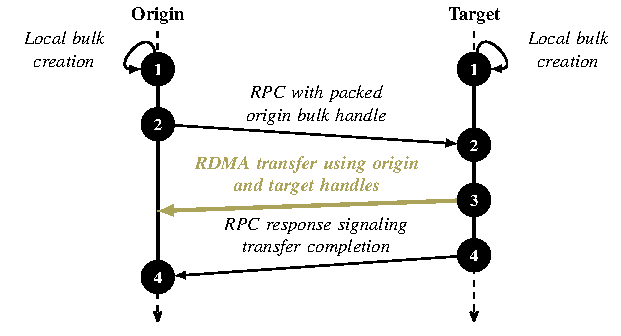
\includegraphics{figs/bulk_rdma}
\vspace{-5pt}
\caption{Four-step process of Mercury's bulk RDMA transfers.}
\label{fig:bulk_rdma}
\vspace{-10pt}
\end{figure}

Enabling RMA capabilities through Mercury's bulk component (see Figure~\ref{fig:overview})
is a four-step process (see Figure~\ref{fig:bulk_rdma}).
First, \textit{bulk handles}, which are abstract memory
descriptors, must be created on both origin and target processes. During
handle creation, memory regions are registered (which in most cases
corresponds to a physical hardware registration); this allows for the
higher level data service to only expose memory pages that it wishes to access in either
read-write or read-only mode. Second, an RPC is issued from the origin
process to the target process with the serialized bulk handle of the origin process;
this handshake allows the target process to gather virtual address information,
registration keys, and so forth, which are necessary for the underlying protocol to post
an RDMA operation.
Third, the actual RDMA operation is posted using both the target's local bulk handle
and the origin's handle that was transmitted through the RPC. Since bulk handles are
abstract memory descriptors, more complex scenarios such as scatter/gather can
be transparently implemented and even delegated to the hardware if the hardware provides this support,
allowing for more efficient transfers. Finally, the RPC response is sent, effectively 
signaling the origin of the transfer completion. This server-driven four-step process is
the most conventional model for data transfers in Mercury, but client-driven transfers are legal
as well. The former is
more commonly recommended for two reasons. First, it enables servers to throttle or
re-order
transfers according to load.  Second, it makes the clients lighter weight and more scalable,
since they do not have to track the state of server resources.

\paragraph{Evaluation.}
To show the importance of supporting this capability, we compare the RPC performance and ``RPC with bulk'' performance
on an InfiniBand cluster (Cooley) that is equipped with 4X FDR Infiniband cards (56 Gb/s).
Compared to TCP over the same network,
our approach improves RPC throughput with close to
$9\times10^{5}$ operations per second and close to 6,000 MB/s average throughput when performing RPC and bulk transfer through the native verbs interface.
Note that the previous results do not use any multi-threading capabilities. We maintain
a number of 32 RPCs in-flight to ensure sustained performance. Multi-threading support is
discussed in the next section.

\begin{figure*}[h]
\subfloat[RPC round-trip benchmark (32 RPCs in-flight).\label{fig:rpc_rate_verbs}]{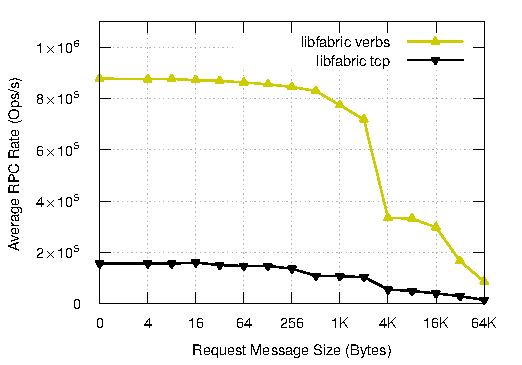
\includegraphics[width=0.49\linewidth]{figs/rpc_rate_verbs} }
\subfloat[Bulk transfer (server pull) benchmark (32 RPC in-flight).\label{fig:write_bw_verbs}]{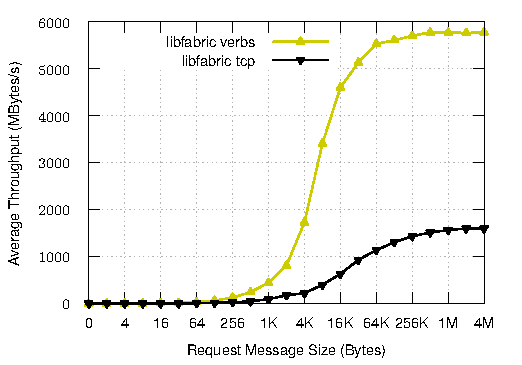
\includegraphics[width=0.49\linewidth]{figs/write_bw_verbs} }
\caption{Effect of leveraging RDMA network on InfiniBand cluster (FDR InfiniBand).}
\label{fig:bench_verbs}
\end{figure*}

\subsection{Multi-Core Architecture Support}
\label{sec:local_scaling}

With CPUs experiencing increasing core count and lower frequencies per
core, data services are expected to take advantage of these architectures
by either distributing the load of incoming RPCs across cores or by
running multiple services co-located within the same node.
% One of the points that we have not detailed so far is Mercury's progress model.
%
Communication
frameworks typically adopt one of two progress models: either \textit{explicit} or
\textit{implicit}. \textit{Explicit} progress implies that the user will regularly
make progress calls to effectively check into network completion queues, poll
file descriptors, etc. In contrast, an \textit{implicit} progress model will 
make progress in background without any need for the user to be involved.
However, this usually involves a background progress thread 
running to make progress while operations are being posted. While
this may seem convenient, this ``hidden'' thread can become detrimental when
running concurrently with other user's threads, leading to unexpected scheduling
issues.
%
Therefore, to prevent this type of issues and give data services sufficient
flexibility in how progress is ensured, we follow an explicit progress
model.
%
RPC is not only about messaging and communication, it is also about
execution of user-defined function calls. When making progress, therefore, it is
often desirable to decouple the RPC execution activities from the network progress activities,
which leads us to actually adopt a \textit{progress-and-trigger} model
that gives services more control over the placement of the progress and
execution threads.
%
In this approach, implicit progress can be accomplished
by the user by having a thread calling progress in background. 

In a typical scenario, an RPC listener service will start posting RPC receive
operations with memory bound to the thread posting the operations.
%
Distributing the execution of these incoming RPCs across multiple threads
(e.g., using a thread pool) can lead to several context switches
at a significant performance penalty. To prevent this scenario, take
advantage of multi-core architectures, and allow for node-local service scaling
without costly creation of separate endpoints per thread, we make
use of \textit{scalable endpoints} (SEP) when available.
%
Scalable endpoints are provided through libfabric~\cite{Grun2015} but
can be extended through our network abstraction layer.
Scalable endpoints allow for
sharing a single endpoint resources between threads by assigning separate
transmit and receive contexts (including completion queues) to each thread. When SEPs
are used, context switches between threads no longer exist---
a fundamental advantage for RPC multi-core architectures.


\begin{figure*}[h]
\subfloat[RPC round-trip benchmark (32 RPCs in-flight).\label{fig:rpc_sep_gni}]{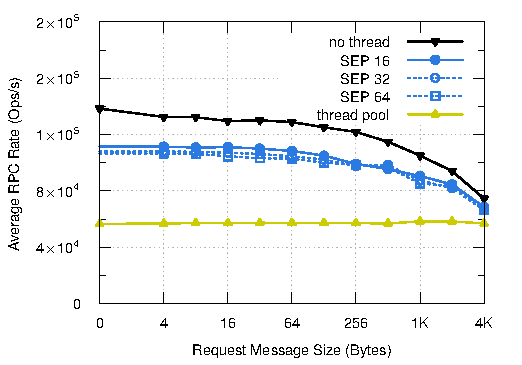
\includegraphics[width=0.49\linewidth]{figs/rpc_rate_sep_gni} }
\subfloat[Bulk transfer benchmark (32 RPC in-flight).\label{fig:write_bw_sep_gni}]{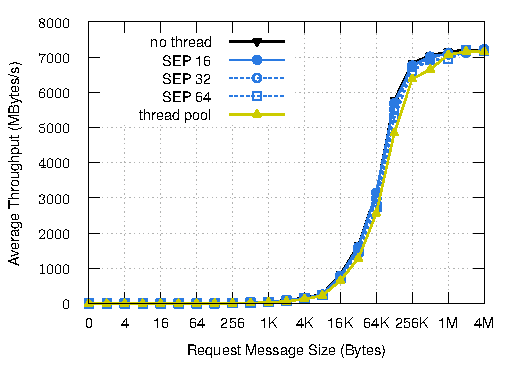
\includegraphics[width=0.49\linewidth]{figs/write_bw_sep_gni} }
\caption{Effect of using scalable endpoints on Cray XC40 (Aries interconnect).}
\label{fig:bench_sep_gni}
\end{figure*}

%\begin{figure*}[h]
%\begin{subfigure}[b]{.49\linewidth}
%\centering
%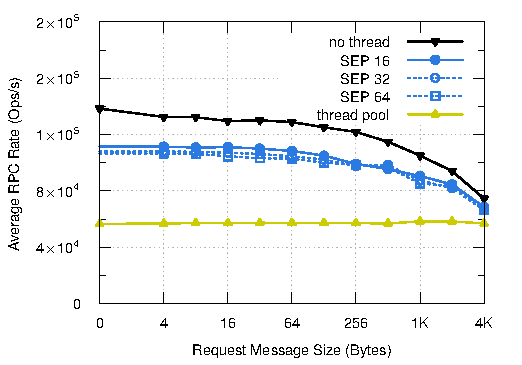
\includegraphics[width=\textwidth]{figs/rpc_rate_sep_gni}
%\caption{RPC round-trip benchmark (32 RPCs in-flight).}
%\label{fig:rpc_rate_sep_gni}
%\end{subfigure}%
%\hfill
%\begin{subfigure}[b]{.49\linewidth}
%\centering
%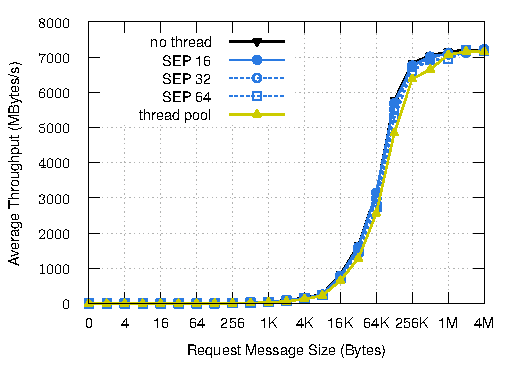
\includegraphics[width=\textwidth]{figs/write_bw_sep_gni}
%\caption{Bulk transfer benchmark (32 RPCs in-flight).}
%\label{fig:write_bw_sep_gni}
%\end{subfigure}
%\vspace{-5pt}
%\caption{Effect of using scalable endpoints on Cray XC40 (Aries interconnect).}
%\label{fig:bench_sep_gni}
%\vspace{-15pt}
%\end{figure*}

\paragraph{Evaluation.} To demonstrate the impact of context switches
and emphasize the benefits of scalable endpoints, we run two
benchmarks on the Theta supercomputer at the Argonne Leadership Computing Facility (ALCF).
Theta is a Cray XC40 system with a second-generation Intel Xeon Phi processor and
Cray Aries interconnect. Each compute node is a single Xeon Phi chip with 64 cores,
16 GB of Multi-Channel DRAM (MCDRAM), and 192 GB of DDR4 memory.
Users typically take advantage of this architecture by either deploying
multiple data services locally or by distributing incoming RPCs across cores.
%
In order to do so using SEP, we assign each core
to make progress and trigger calls on their own receive context.
As shown in Figure~\ref{fig:bench_sep_gni}, using SEP provides
close match (in terms of operations per second) to the performance of workloads
that do not use multi-threading. 
%
Distributing requests using a thread pool, in contrast, has a significant
detrimental impact on RPC rate.  Note that in all cases bulk transfers
exhibit similar overall bandwidth, as context switches only represent a
portion of the time spent when large data is transferred over the network.

\subsection{Flexible Provisioning and Topology}
\label{sec:local_deployment}

In the preceding section, we demonstrated node-level scaling when RPCs are made between
separate nodes using the native interconnect. Additional optimization can be made,
however, by being aware of node-local process placement, in order to ensure efficient
composition of services.

\subsubsection{Transparent Node-Local Deployment}

When deploying data
services, it is common for some of these services to either issue
RPCs to other local services (i.e., separate processes within the same node) or
to send RPCs back to themselves (i.e., within the same process).
The latter typically arises out of convenience, rather than creating a separate code path for
that case.
To achieve the former,
Mercury can make use of shared-memory transparently by detecting that
the target address is on the same node. Using lockless shared ring buffers and
lockless queues, it is possible to achieve lockless transfers with very low
latency. For bulk data transfers and to prevent any intermediate \textit{memcpy},
zero-copy transfers (i.e, one single and direct copy from origin to target buffer) can be
achieved using the Linux Cross-Memory Attach mechanism.

To achieve the latter, Mercury detects when the target address is the
same as the origin address and sends RPCs using the same argument packing mechanism,
by immediately queuing the RPC into a local completion queue, internally signaling
completion to wake up any potential thread waiting in a progress call. Likewise,
bulk data transfers are realized through a \textit{memcpy} between source and
destination buffers.

This combination of transparent shared-memory transfers between separate processes,
loopback redirection within the same process, and over-the-wire transfers has
shown substantial benefits when deploying data services in terms of performance
and flexibility, since data services can treat all three scenarios identically.


\begin{figure*}[h]
\subfloat[RPC round-trip benchmark (32 RPCs in-flight).\label{fig:rpc_rate_sm}]{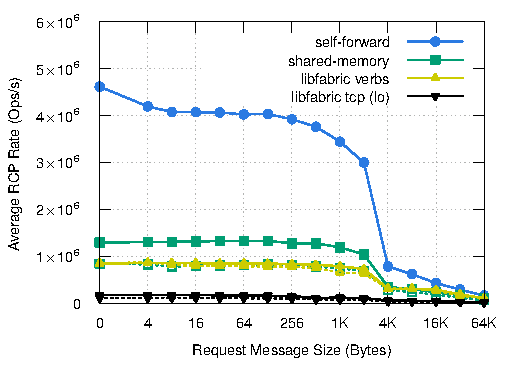
\includegraphics[width=0.49\linewidth]{figs/rpc_rate_sm} }
\subfloat[Bulk transfer benchmark (32 RPC in-flight).\label{fig:write_bw_sm}]{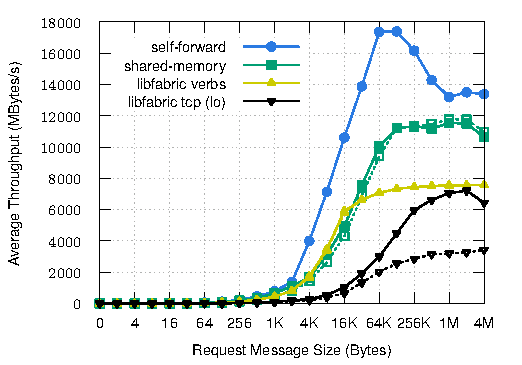
\includegraphics[width=0.49\linewidth]{figs/write_bw_sm} }
\caption{Comparison between node-local RPC mechanisms on InfiniBand cluster (FDR InfiniBand).}
\label{fig:bench_sm}
\end{figure*}

%\begin{figure*}[h]
%\begin{subfigure}[b]{.5\linewidth}
%\centering
%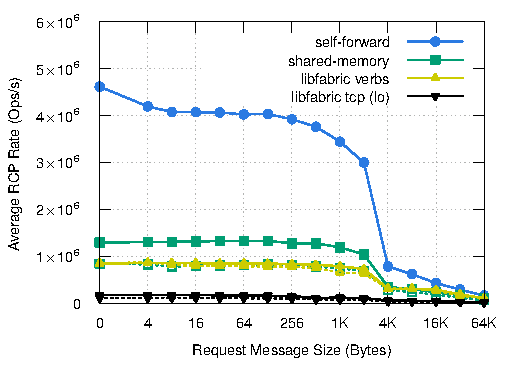
\includegraphics[width=\textwidth]{figs/rpc_rate_sm}
%\caption{RPC round-trip benchmark (32 RPCs in-flight).}
%\label{fig:rpc_rate_sm}
%\end{subfigure}%
%\hfill
%\begin{subfigure}[b]{.5\linewidth}
%\centering
%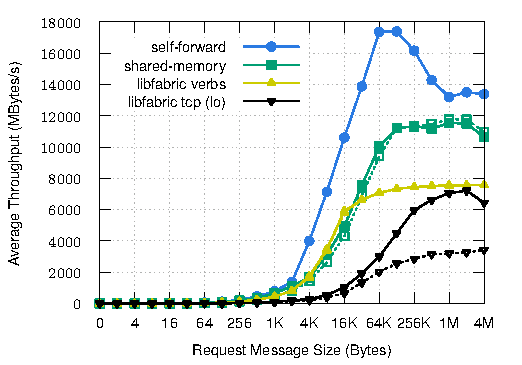
\includegraphics[width=\textwidth]{figs/write_bw_sm}
%\caption{Bulk transfer (server pull) benchmark (32 RPCs in-flight).}
%\label{fig:write_bw_sm}
%\end{subfigure}
%\vspace{-5pt}
%\caption{Comparison between node-local RPC mechanisms on InfiniBand cluster (FDR InfiniBand).}
%\label{fig:bench_sm}
%\vspace{-10pt}
%\end{figure*}

\paragraph{Evaluation.} To illustrate this scenario on our InfiniBand cluster (Cooley),
we compare in  Figure~\ref{fig:bench_sm} our two local RPC communication mechanisms 
to issuing RPCs either through the native interconnect (in this case InfiniBand Verbs)
or through TCP and the loopback interface. The latter is one of the fallback 
mechanisms typically used when not using shared-memory.
Cooley is equipped of dual-sockets nodes with Intel Xeon E5-2620 v3 CPUs. Consequently,
performance varies depending on process placement and the NUMA nodes being used---performance when running on separate NUMA nodes is represented by a dotted line in Figure~\ref{fig:bench_sm}.
In terms of both RPC
operations per second and bulk throughput, these two mechanisms are very valuable,
providing much better performance than both the native interconnect and TCP
(1.3 MOps/s for shared-memory and more than 4 MOps/s for loopback execution).
When running on separate NUMA nodes, shared-memory performance is naturally
impacted, though RPCs with bulk transfer still perform at a much higher rate due to the use
of Linux Cross-Memory Attach (CMA).

\subsubsection{Service Composition}

With node-level scaling and transparent node-local deployment in place,
composing data services seems the next natural step. In order to provide flexible composition, 
the RPC API must not be specific to any implementation but rather rely only on \textit{origin} and
\textit{target} concepts. The RPC mechanism then can be consistently employed to communicate
between different service ``servers'' and ``clients''.

\begin{figure}[h]
\centering
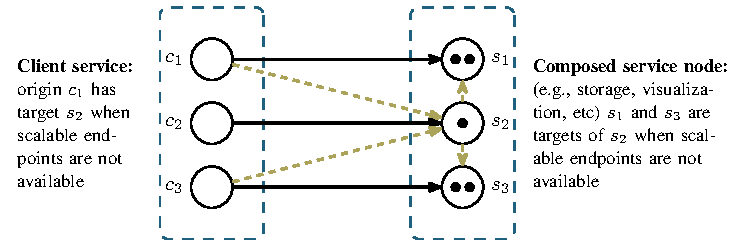
\includegraphics{figs/composition}
\caption{Composition of services with and without scalable endpoints.}
\label{fig:composition}
%\vspace{-5pt}
\end{figure}

When multiple services are colocated, there is also a need for addressing specific services and 
efficiently making progress. 
%
As shown in Figure~\ref{fig:composition}, this can then be accomplished by
using a ``delegator'' service, which can potentially become a bottleneck,
or by using scalable endpoints addressing specific receive contexts
directly through an ID that can be defined for each data service.
%
When there is no hardware support for scalable endpoints, however, this
functionality must be emulated by embedding a service ID into the RPC
header and using that ID to distribute RPC requests to the corresponding
service through that delegator.  An alternative is to create multiple
endpoints, one for each data service; but this is usually not recommended
due to hardware resource limitations.

\subsection{Multi-Network Support}

As we bridge local and nonlocal communication mechanisms, supporting multiple
fabrics follows a similar approach and relies on the same supporting
components described in Sections~\ref{sec:local_scaling} 
and~\ref{sec:local_deployment}. Mercury's architecture defines \textit{classes}
that physically correspond to one endpoint and \textit{contexts} that correspond
to completion queues and locally allocated resources. When using scalable endpoints
as described in Section~\ref{sec:local_scaling}, we are in a scenario with one class
(one endpoint) and multiple contexts (multiple completion queues) that share the same
endpoint. When bridging multiple fabrics, we are in a scenario with multiple classes 
(multiple endpoints) and one or more contexts (completion queues) associated with
each class.

The challenge is efficiently making progress over these separate
classes and contexts. To facilitate this, Mercury provides two progress
mechanisms, allowing for a service to either
%
busy spin on each of these contexts to process requests as quickly as possible (at the cost
of using more CPU resources), or to
%
wait and sleep on this set of contexts until a new request arrives.
%
In the latter case, we rely on Linux' file descriptor and \textit{epoll}
mechanism to wait. This allows for monitoring of both local event
notifications and hardware queue notifications. This transparent
notification mechanism allows a data service implementation to
simply wait on a file descriptor rather than manually making progress
on each of the interfaces/endpoints.

\subsection{Resilience and Fault Tolerance}
\label{sec:cb}

When supporting data services at scale, there are multiple approaches that one can take
to define a resilient RPC mechanism (for instance, guaranteed delivery).
One of the primary requirements for an RPC component is to allow services to
recover after a fault has occurred (e.g., node failure, unresponsiveness of a
service component) without compromising performance, by simply providing
robust support for canceling operations that are pending.
This implies reclaiming local resources that RPC operations have previously
allocated and gracefully recovering from faults.
It is important to note that we assume in that discussion the use of
\textit{reliable} unconnected endpoints in the transport layer, hence RPC requests
do not get ``lost''. Ordering and tag matching are not
critical for the transport to provide though (Mercury matches messages itself when needed).
Mercury itself only provides \textit{at-most} once semantics: nonblocking RPC
requests are sent and a nonblocking response is sent back (unless it is explicitly stated 
not to do so). It is then up to services to make their
own decision on how to react (e.g., retry, fail over, initiate a rebuild, etc).
Both RPC and bulk data transfer operations may be interrupted if any of the
peers involved no longer responds, in which case pending operations must be
canceled. Canceling an operation that cannot
complete, either because a fault has occurred or a timeout has been reached, 
is necessary in order to reach proper completion.

\begin{figure}[h]
\centering
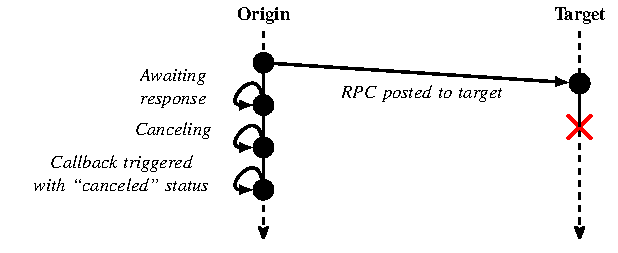
\includegraphics{figs/cancel}
%\vspace{-5pt}
\caption{Cancelation of an RPC operation.}
\label{fig:cancel}
%\vspace{-5pt}
\end{figure}

Cancelation of operations in Mercury is always an \textit{asynchronous} and
\textit{local} operation. As shown in Figure~\ref{fig:cancel}, forwarding an RPC
request is a nonblocking operation. Therefore, since Mercury follows a callback-based
mechanism, completion of that operation is known from a user's
perspective only when the callback that is associated to that operation
is pushed to the local completion queue and later triggered after making both
progress and trigger calls. When that callback is triggered, the state of the
operation is reported to the user as \textit{canceled}. Since operations are nonblocking,
keeping cancelation an asynchronous operation instead of an operation that completes
immediately is essential.
This mechanism protects against races in the event that a peer response arrives
after local cancelation has already succeeded. After the callback is triggered,
it is then safe to re-use the existing RPC request handle to issue a retry for example.

Cancelation is the foundation for implementing timeout scenarios in data services
in order to recover from a fault. When an internal
fault occurs, however, cancelation of the operation is not always necessary if the RPC
has not yet been posted, in which case that operation can simply be directly retried. This
scenario is similar for all other nonblocking operations in Mercury, including
bulk data transfers.

\section{Applications and Use Cases}
\label{sec:apps}

As mentioned in Section~\ref{sec:intro}, Mercury is part of the Mochi suite of service of components.
Mochi provides additional features on top of Mercury such as the notion of group membership,
transparent user-level thread semantics, key/value stores, C++ and Python bindings.
This work is further described in~\cite{Ross2020} along with
additional use cases, including the following:

Intel's \textit{Distributed Application Object Storage} (DAOS)~\cite{Intel2019} project
provides a transactional and multidimensional object store for
use in large-scale HPC environments with embedded storage directly
attached to the compute fabric. DAOS is a vendor-backed push to
provide an alternative to the traditional parallel file system and has the
potential to extract higher performance out of emerging low latency storage
technology by running in user space. DAOS is envisioned as a multiuser and persistent
volume available to all applications. It therefore encompasses a variety of
system management capabilities, including distributed authentication and
device provisioning.

The \textit{Unify} project, the successor to BurstFS~\cite{Wang2016},
implements a temporary high-performance file system using
local resources on nodes in the HPC system. In Unify, data is
explicitly staged between the temporary Unify file system and the
``permanent'' parallel file system. The Unify team is exploring
specialization in the form of multiple flavors of file systems, such
as \textit{UnifyCR} for
checkpoint/restart workloads and a
separate specialized version for machine learning workloads. This backend
specialization allows Unify to optimize for different use cases without
sacrificing the portability and common toolset advantages of a POSIX
interface. UnifyCR, for example, uses user-space I/O interception,
scalable metadata indexing, and colocated I/O delegation to optimize
bursty checkpoint workloads while still presenting a traditional file
system view of the data.

\textit{GekkoFS}~\cite{Vef2018} implements a temporary and
highly scalable file system providing relaxed POSIX semantics tailored
to the majority of HPC applications. This type of specialization
allows applications using the existing POSIX interface (under
specific constraints) to see dramatic performance improvements
as compared with file systems supporting the complete specification. The
GekkoFS team has demonstrated millions of metadata operations per
second, allowing it to serve applications with access patterns that
were historically poor matches for file systems, and the team has shown rapid
service instantiation times allowing new GekkoFS volumes to be started
on a per-job basis.

\textit{Proactive Data Containers} (PDC)~\cite{Mu2018} provides a data
model in which a container holds a collection of objects that may
reside at different levels of a potentially complex storage hierarchy and
migrate between them. A PDC volume is instantiated for an application
workflow and sized to meet workflow requirements for data storage
and I/O. Objects can hold both streams of bytes and KV pairs,
and additional metadata can be associated with objects as well.
Unlike GekkoFS and UnifyCR, PDC does not present a conventional file
system interface but instead provides a way of unifying application's memory
and storage by providing object mapping semantics, which hide actual I/O transfers
between storage hierarchies from the user.

\section{Conclusion}
\label{sec:concl}

To support data services at scale, a re-usable RPC component must be able
to provide performance by enabling the use of all the underlying hardware and
network fabrics, flexibility by facilitating service composition, and resilience
by providing support for local cancelation. Mercury in that regard is
already providing this functionality and is on the path of being used on
production systems, to enable not only file system capabilities but to also
provide specialized data service workflows as part of the Mochi suite of
components.

We are also considering how to make use of
collectives through Mercury and how to provide data services with
optimized collective RPC operations (such as RPC broadcasts) that do not only
rely on point-to-point messaging, which is a limitation when an RPC
must be sent to a large number of targets.
Furthermore, with accelerators (e.g., GPUs) that are now part of the HPC ecosystem, there
is a growing interest in how to make efficient use of RDMA and address the accelerator's 
memory directly from a remote target. These are two future directions
that we are considering to further evolve our RPC framework.

\section*{Acknowledgments}

This material was based upon work supported in part by the U.S. Department
of Energy, Office of Science, Advanced Scientific Computing Research
program, under Contract No. DE-AC02-06CH11357; in part supported by
the Exascale Computing Project (17-SC-20-SC), a joint project of the
U.S. Department of Energy`s Office of Science and National Nuclear
Security Administration.  responsible for delivering a capable exascale
ecosystem, including software, applications, and hardware technology,
to support the nation`s exascale computing imperative; and in part
supported by the U.S. Department of Energy, Office of Science, Office
of Advanced Scientific Computing Research, Scientific Discovery through
Advanced Computing (SciDAC) program.

This research used resources of the Argonne Leadership Computing
Facility, which is a DOE Office of Science User Facility supported
under Contract DE-AC02-06CH11357.

The authors would like to thank Howard Pritchard for his help on
successfully porting this software to Cray GNI-based systems.

\begin{thebibliography}{10}
\itemsep=1pt
\begin{small}

\bibitem{mpich}
{Argonne National Laboratory}, ``{MPICH},'' 2013. [Online]. Available:
  \url{http://www.mpich.org}

\bibitem{Zounmevo2013}
J.~Zounmevo, D.~Kimpe, R.~Ross, and A.~Afsahi, ``{On the Use of MPI in
  High-Performance Computing Services},'' in \emph{Recent Advances in the
  Message Passing Interface}, 2013.

\bibitem{protobuf}
{Google Inc}, ``{Protocol Buffers},'' 2012. [Online]. Available:
  \url{https://developers.google.com/protocol-buffers}

\bibitem{Slee2007}
M.~Slee, A.~Agarwal, and M.~Kwiatkowski, ``{Thrift: Scalable Cross-Language
  Services Implementation},'' Facebook, 156 University Ave, Palo Alto, CA,
  Tech. Rep., 2007.

\bibitem{Wang2009}
F.~Wang, S.~Oral, G.~Shipman, O.~Drokin, T.~Wang, and I.~Huang,
  ``{Understanding Lustre Filesystem Internals},'' Oak Ridge National Lab.,
  National Center for Computational Sciences, Tech. Rep., 2009,
  {O}RNL/TM-2009/117.

\bibitem{Welch2008}
B.~Welch, M.~Unangst, Z.~Abbasi, G.~Gibson, B.~Mueller, J.~Small, J.~Zelenka,
  and B.~Zhou, ``{Scalable Performance of the Panasas Parallel File System},''
  in \emph{Proceedings of the 6th USENIX Conference on File and Storage
  Technologies}, ser. FAST’08.\hskip 1em plus 0.5em minus 0.4em\relax USA:
  USENIX Association, 2008.

\bibitem{Ali2009}
N.~Ali, P.~Carns, K.~Iskra, D.~Kimpe, S.~Lang, R.~Latham, R.~Ross, L.~Ward, and
  P.~Sadayappan, ``{Scalable I/O Forwarding Framework for High-Performance
  Computing Systems},'' in \emph{IEEE International Conference on Cluster
  Computing and Workshops}, 2009, pp. 1--10.

\bibitem{Sandberg1988}
R.~Sandberg, D.~Golgberg, S.~Kleiman, D.~Walsh, and B.~Lyon, \emph{Design and
  Implementation of the Sun Network Filesystem}.\hskip 1em plus 0.5em minus
  0.4em\relax USA: Artech House, Inc., 1988, pp. 379--390.

\bibitem{Soumagne2013}
J.~{Soumagne}, D.~{Kimpe}, J.~{Zounmevo}, M.~{Chaarawi}, Q.~{Koziol},
  A.~{Afsahi}, and R.~{Ross}, ``{Mercury: Enabling Remote Procedure Call for
  High-Performance Computing},'' in \emph{2013 IEEE International Conference on
  Cluster Computing (CLUSTER)}, Sep. 2013, pp. 1--8.

\bibitem{Ross2020}
R.~B. Ross, G.~Amvrosiadis, P.~Carns, C.~D. Cranor, M.~Dorier, K.~Harms,
  G.~Ganger, G.~Gibson, S.~K. Gutierrez, R.~Latham, B.~Robey, D.~Robinson,
  B.~Settlemyer, G.~Shipman, S.~Snyder, J.~Soumagne, and Q.~Zheng, ``{Mochi:
  Composing Data Services for High-Performance Computing Environments},''
  \emph{Journal of Computer Science and Technology}, vol.~35, no.~1, pp.
  121--144, Jan 2020. [Online]. Available:
  \url{https://doi.org/10.1007/s11390-020-9802-0}

\bibitem{Docan2012}
C.~Docan, M.~Parashar, and S.~Klasky, ``{DataSpaces: An Interaction and
  Coordination Framework for Coupled Simulation Workflows},'' \emph{Cluster
  Computing}, vol.~15, no.~2, pp. 163--181, Jun. 2012. [Online]. Available:
  \url{https://doi.org/10.1007/s10586-011-0162-y}

\bibitem{Docan2010}
------, ``{Enabling High-speed Asynchronous Data Extraction and Transfer Using
  DART},'' \emph{Concurr. Comput. : Pract. Exper.}, vol.~22, no.~9, pp.
  1181--1204, 2010.

\bibitem{Wood2016}
C.~Wood, S.~Sane, D.~Ellsworth, A.~Gimenez, K.~Huck, T.~Gamblin, and A.~Malony,
  ``"a scalable observation system for introspection and in situ analytics",''
  in \emph{Proceedings of the 5th Workshop on Extreme-Scale Programming Tools},
  ser. ESPT ’16.\hskip 1em plus 0.5em minus 0.4em\relax IEEE Press, 2016, pp.
  42--49.

\bibitem{Ulmer2018}
C.~Ulmer, S.~Mukherjee, G.~Templet, S.~Levy, J.~Lofstead, P.~Widener,
  T.~Kordenbrock, and M.~Lawson, ``"faodel: Data management for next-generation
  application workflows",'' in \emph{Proceedings of the 9th Workshop on
  Scientific Cloud Computing}, ser. ScienceCloud’18.\hskip 1em plus 0.5em
  minus 0.4em\relax New York, NY, USA: Association for Computing Machinery,
  2018. [Online]. Available: \url{https://doi.org/10.1145/3217880.3217888}

\bibitem{Lofstead2011}
J.~Lofstead, R.~Oldfield, T.~Kordenbrock, and C.~Reiss, ``{Extending
  Scalability of Collective IO through Nessie and Staging},'' in
  \emph{Proceedings of the Sixth Workshop on Parallel Data Storage}.\hskip 1em
  plus 0.5em minus 0.4em\relax New York, NY, USA: ACM, 2011, pp. 7--12.

\bibitem{Grun2015}
P.~{Grun}, S.~{Hefty}, S.~{Sur}, D.~{Goodell}, R.~D. {Russell}, H.~{Pritchard},
  and J.~M. {Squyres}, ``{A Brief Introduction to the OpenFabrics Interfaces -
  A New Network API for Maximizing High Performance Application Efficiency},''
  in \emph{2015 IEEE 23rd Annual Symposium on High-Performance Interconnects},
  Aug 2015, pp. 34--39.

\bibitem{Intel2019}
{Intel Corporation}, ``{DAOS: Revolutionizing High-Performance Storage with
  Intel Optane Technology},''
  \url{https://www.intel.com/content/dam/www/public/us/en/documents/solution-briefs/high-performance-storage-brief.pdf},
  Jun. 2019.

\bibitem{Wang2016}
T.~{Wang}, K.~{Mohror}, A.~{Moody}, K.~{Sato}, and W.~{Yu}, ``{An Ephemeral
  Burst-Buffer File System for Scientific Applications},'' in \emph{SC '16:
  Proceedings of the International Conference for High Performance Computing,
  Networking, Storage and Analysis}, Nov 2016, pp. 807--818.

\bibitem{Vef2018}
M.~{Vef}, N.~{Moti}, T.~{Süß}, T.~{Tocci}, R.~{Nou}, A.~{Miranda},
  T.~{Cortes}, and A.~{Brinkmann}, ``{GekkoFS---A Temporary Distributed File
  System for HPC Applications},'' in \emph{2018 IEEE International Conference
  on Cluster Computing (CLUSTER)}, Sep. 2018, pp. 319--324.

\bibitem{Mu2018}
J.~{Mu}, J.~{Soumagne}, H.~{Tang}, S.~{Byna}, Q.~{Koziol}, and R.~{Warren},
  ``{A Transparent Server-Managed Object Storage System for HPC},'' in
  \emph{2018 IEEE International Conference on Cluster Computing (CLUSTER)},
  Sep. 2018, pp. 477--481.

\end{small}
\end{thebibliography}

\end{document}
